\chapter{Graceful Numbering}

Rishnak found Ajur and Jura playing near the water fountain. Continuing the conversation from the previous day, Rishnak reminded Ajur about vertex coloring and edge coloring as types of graph labeling schemes with constraints defined such that adjacent vertices and edges are not colored the same.

Rishnak said, ``There are other labeling schemes. One such scheme in particular is called the \textit{graceful numbering} of a graph. Given graph~$G=(V,E)$ with~$n$ vertices and~$e$ edges, we assign distinct numbers to the vertices from~$0,1,2,\ldots,e$ such that all edge labels are distinct from~$1,2,\ldots,e$. The edge label is the absolute value of the difference between the numbers associated with the end vertices.''

\begin{figure}
\begin{center}
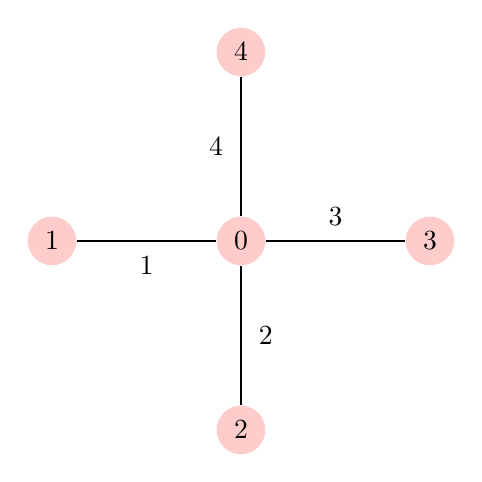
\begin{tikzpicture}
  [scale=.6,auto=left,every node/.style={circle,fill=red!20}]
  \tikzstyle{weight} = [fill=none]
  \node (n1) at (5,5) {0};
  \node (n2) at (1,5)  {1};
  \node (n3) at (5,1)  {2};
  \node (n4) at (9,5) {3};
  \node (n5) at (5,9)  {4};
\foreach \source /\dest /\weight in {n1/n2/1,n1/n3/2,n1/n4/3,n1/n5/4} 
   \draw (\source) --node[weight] {$\weight$}  (\dest);

\end{tikzpicture}
\caption{A star tree that is gracefully numbered since each of the edges has a distinct weight that is the absolute value of the difference between the endpoint vertex labels}\label{19g1}
\end{center}
\end{figure}

Ajur scratched his head, so Rishnak waved his hands and a graph appeared [Figure~\ref{19g1}].

Rishnak said, ``Here is an example of a star tree. It consists of a center vertex connected to many leaves.  Each edge weight is the absolute value of the difference between the two endpoint vertex labels. Can you draw such a graph that is a simple path of six vertices?''

Ajur picked up a stick and tried to draw such a graph in the dirt [Figure~\ref{19g2}].  He smiled and said, ``Yes, here is a gracefully numbered graph for a path of length~5.''

Rishnak smiled and said, ``Good, Ajur. And like a star tree, your snake graph can also be generalized to an arbitrary number of vertices.\footnote{Can you generalize each of these problems?} Next, try a binary tree with seven vertices.''

\begin{figure}
\begin{center}
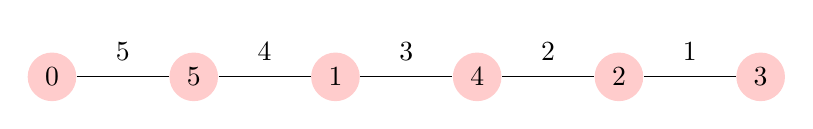
\begin{tikzpicture}
  [scale=.6,auto=left,every node/.style={circle,fill=red!20}]
  \tikzstyle{weight} = [fill=none]
  \node (n1) at (1,1) {0};
  \node (n2) at (4,1)  {5};
  \node (n3) at (7,1)  {1};
  \node (n4) at (10,1) {4};
  \node (n5) at (13,1)  {2};
  \node (n6) at (16,1) {3};
\foreach \source /\dest /\weight in {n1/n2/5,n2/n3/4,n3/n4/3,n4/n5/2,n5/n6/1} 
   \draw (\source) --node[weight] {$\weight$}  (\dest);


\end{tikzpicture}
\caption{A gracefully numbered path (snake) in which each of the edges has a distinct number that is the absolute value of the difference between the labels of the endpoint vertices}\label{19g2}
\end{center}
\end{figure}

Ajur drew a binary tree with seven vertices in the dirt, then slowly labeled each vertex and each edge [Figure~\ref{19g3}]. He said, ``Here is a graceful numbering!''

\begin{figure}
\begin{center}

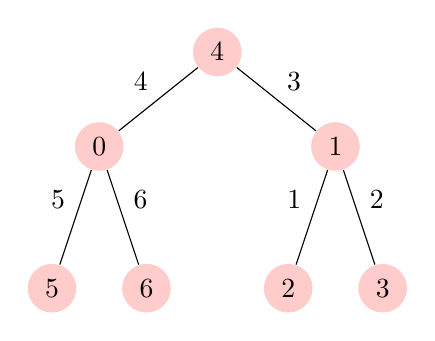
\begin{tikzpicture}
  [scale=.6,auto=left,every node/.style={circle,fill=red!20}]
  \tikzstyle{weight} = [fill=none]
  \node (n1) at (5.5,7) {4};
  \node (n2) at (3,5)  {0};
  \node (n3) at (8,5)  {1};
  \node (n4) at (2,2) {5};
  \node (n5) at (4,2)  {6};
  \node (n6) at (7,2)  {2};
  \node (n7) at (9,2)  {3};
\foreach \source /\dest /\weight in {n2/n1/4,n1/n3/3,n4/n2/5,n2/n5/6,n6/n3/1,n3/n7/2} 
   \draw (\source) --node[weight] {$\weight$}  (\dest);
  
\end{tikzpicture}

\caption{A gracefully numbered binary tree with seven vertices}\label{19g3}
\end{center}
\end{figure}

Rishnak said, ``It is not known whether all binary trees have a graceful numbering. This is one of many open questions in graph theory. Attempts have been made to find counterexamples---meaning trees that do not have a graceful numbering---but these attempts have failed. And efforts to find a proof to show that all binary trees have a graceful numbering have also failed.''

Ajur wondered at this, then said, ``Are there graphs for which we know there is no graceful numbering?''

Rishnak said, ``There are graphs that do not have a graceful numbering''---he flashed his hands and a new graph appeared [Figure~\ref{19g4}]---``such as this graph with a cycle of length~5.''

\begin{figure}
\begin{center}

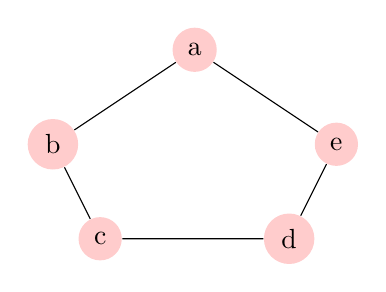
\begin{tikzpicture}
  [scale=.6,auto=left,every node/.style={circle,fill=red!20}]

  \node (n1) at (4,1) {a};
  \node (n2) at (1,-1)  {b};
  \node (n3) at (2,-3)  {c};
  \node (n4) at (6,-3) {d};
  \node (n5) at (7,-1)  {e};
 
\foreach \from/\to in {n1/n2,n2/n3,n3/n4,n4/n5,n5/n1}
    \draw (\from) -- (\to);
  
\end{tikzpicture}

\caption{The~$C_5$ graph (cycle of length~5) for which we cannot come up with a graceful numbering}\label{19g4}
\end{center}
\end{figure}

Rishnak continued, ``Complete bipartite graph~$K_{m,m}$ can be gracefully numbered (or colored) by numbering vertices in one partition~$0,1,\ldots,m-1$ and numbering vertices in the other partition~$m,2m,3m,\ldots,m^2$. With this numbering all of the edges get distinct numbers that meet the requirements of a gracefully numbered graph. Here, Ajur, try this for~$m=3$.''

Ajur thought about this for a minute. He knew the~$K_{3,3}$ graph must have six vertices, with three vertices in each partition, but how should they be numbered? He tried a few possibilities in his head, then drew a bipartite graph in the dirt and labeled its vertices and edges [Figure~\ref{18g45}].

\begin{figure}
\begin{center}

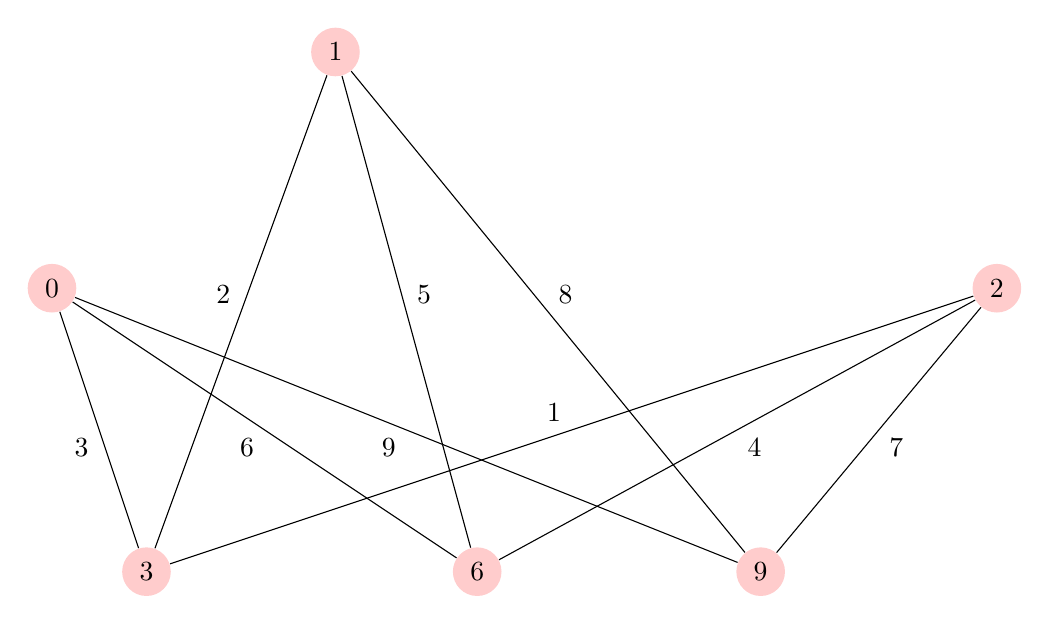
\begin{tikzpicture}
  [scale=.6,auto=left,every node/.style={circle,fill=red!20}]
  \tikzstyle{weight} = [fill=none]
  \node (n1) at (-3,5) {0};
  \node (n2) at (3,10)  {1};
  \node (n3) at (17,5)  {2};
  \node (n4) at (-1,-1) {3};
  \node (n5) at (6, -1) {6};
  \node (n6) at (12,-1)  {9};
 
\foreach \source /\dest /\weight in {n4/n1/3,n5/n1/6,n6/n1/9} 
   \draw (\source) --node[weight] {$\weight$}  (\dest);
\foreach \source /\dest /\weight in {n4/n2/2,n2/n5/5,n2/n6/8} 
   \draw (\source) --node[weight] {$\weight$}  (\dest);
\foreach \source /\dest /\weight in {n4/n3/1,n3/n5/4,n3/n6/7} 
   \draw (\source) --node[weight] {$\weight$}  (\dest);

 
  \end{tikzpicture}
\caption{A gracefully numbered~$K_{3,3}$ graph}\label{18g45}
\end{center}
\end{figure}

Rishnak smiled, pleased to see Ajur's work. Rishnak said, ``One last new concept for you, Ajur. Closely related to graceful numbering, a \textit{Golomb ruler} is an imaginary ruler that has a set of marks at integer positions such that no two pairs of marks are the same distance apart.''

Ajur tried to understand this, repeating it to himself.

After a pause, Rishnak said, ``The number of marks on a Golomb ruler is its \textit{order}, and the largest distance between two of its marks is its \textit{length}. So a Golomb ruler of order~3 has marks~$\{0,1,3\}$ and can be used to measure all lengths up to length~3. A Golomb ruler of order~4 has marks~$\{0,1,4,6\}$ and can measure all lengths up to length~6.''

Ajur hurriedly said, ``I get it.''

Rishnak said, ``The Golomb ruler has applications in coding theory and, it turns out, can be used to gracefully number complete graph~$K_4$, which''---Rishnak flashed his hands and a new graph appeared [Figure~\ref{19g5}]---``I present to you here.''

\begin{figure}
\begin{center}

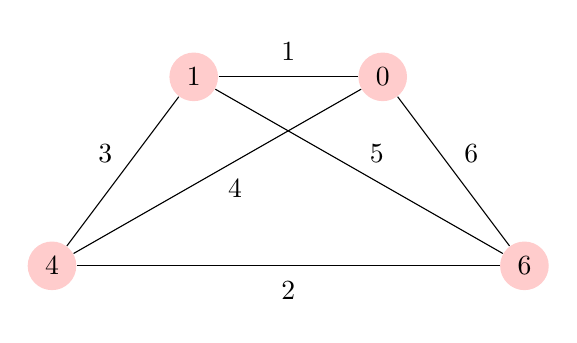
\begin{tikzpicture}
  [scale=.6,auto=left,every node/.style={circle,fill=red!20}]
  \tikzstyle{weight} = [fill=none]
  \node (n1) at (5, -1) {0};
  \node (n2) at (1,-1)  {1};
  \node (n3) at (-2,-5)  {4};
  \node (n4) at (8,-5) {6};

 \foreach \source /\dest /\weight in {n2/n1/1,n1/n3/4,n1/n4/6,n3/n2/3,n2/n4/5,n4/n3/2} 
   \draw (\source) --node[weight] {$\weight$}  (\dest);

\end{tikzpicture}

\caption{Complete graph~$K_4$ gracefully numbered using a Golomb ruler}\label{19g5}
\end{center}
\end{figure}

Ajur studied the graph, understanding after some trial and error that the vertices and edges corresponded to the Golomb ruler lengths.

\subsection*{Question for the seventeenth day}
Seeing that Ajur understood, Rishnak said, ``The questions for the seventeenth day comes from my favorite author, Henry Ernest Dudeney and is Problem~453. It goes something like this. A young studious pupil finds an old yardstick---which you might not know, a yardstick is~36 inches long.
This yardstick is broken in that~3 inches have been chopped clean off, leaving a yardstick that is only~33 inches in length, no longer a yard.''

Ajur laughed as Rishnak continued, ``Some of the graduation marks are also obliterated, leaving only eight such legible marks. Still, this studious pupil is able to measure any length, in inches, from~1 inch to~33 inches. How many ways can you place these eight marks on the broken yardstick?''

Ajur said, ``That doesn't sound too hard.''

Rishnak smiled and said, ``Be careful with this one. It is more difficult than it seems.''

\textit{Before you turn the page, try to come up with answers of your own!}

\newpage
\subsection*{Answer for the seventeenth day}
Ajur quickly saw that this problem was quite similar to the Golomb ruler concept. Excited, Ajur started working on the problem, but an hour passed as Ajur worked. This was more difficult than he had thought.

At last, Ajur said, ``I have~11 solutions and here they are!'' He had sketched them in the dirt:
\begin{itemize}
    \item 1, 2, 3, 4, 10, 16, 22, 28
    \item 1, 2, 3, 4, 10, 17, 22, 28
    \item 1, 2, 3, 8, 14, 20, 24, 29
    \item 1, 2, 3, 10, 15, 22, 27, 31
    \item 1, 2, 3, 10, 16, 21, 25, 29
     \item 1, 2, 3, 11, 17, 21, 26, 30
     \item 1, 2, 3, 14, 18, 23, 25, 29
     \item 1, 2, 3, 14, 18, 23, 26, 29
     \item 1, 2, 3, 16, 21, 22, 26, 30
     \item 1, 2, 3, 16, 21, 24, 27, 31
     \item 1, 2, 4, 11, 18, 25, 30, 31
\end{itemize}

Rishnak raised his eyebrows and said, ``Good, Ajur. I was worried you were stumped. There are more than~50 solutions, but let us call it a day.''

Rishnak noticed that Ajur had used a systematic ``brute force'' technique to solve this problem. Therefore, Rishnak decided to talk about this and more efficient search techniques the next day.

Ajur was tired but pleased to have learned a new type of ruler, one that was connected to graceful numbering.
